\chapter{Data Augmnetation and Segmentation}

\section{Introduction}
This section holds a discussion on segmentation and  techniques producing statistically significant border cut-off at the perimeter of the skin lesion. An accurate border cut-off is an essential criterion for melanoma detection\cite{Pereira2020, Kaya2016} using ABCD rules. Unfortunately, segmentation continues to be a challenging task because datasets regularly contain an estimated border and sometimes an inaccurate border cut-off.

\section{Related Works}
An approach by Albanhli\cite{Albahli2020} uses deep learning-based segmentation algotihm using YOLOv4-arkNet and active countour for melanoa and lesion detection and segmenation. They demonstarted a high accuracy and practicality for clinical decision support systems.

A technique by Seeja R D\cite{seeja2019} uses a convolutional neural network (CNN) based on a U-net algorithm for segmentation based on colour, texture, and shapes to improve image classification.

A technique by Hyunju Lee\cite{Lee2020} uses an edge fill method called u-otsu using the U channel from YUV for segmentation. This is followed by an analysis of ABCD rules, demonstrating the importance of an accurate border cut-off.

\section{Skin Lesion Augmentation}
Skin lesion augmentation is especially vital because of the use of macroscopic images instead of dermoscopic images. This means there are various artefacts including hair, specular reflections, rulers, varying sizes, and shapes of the skin lesion. All of these can obscure the skin lesion and affect the accuracy of segmentation\cite{Unver2019} and in effect feature detection.

By augmenting the skin lesion images using specular reflection removal and hair removal, the accuracy of feature classification methods can be improved\cite{kasmi2023}. 

\subsection{Hair Removal}
Hair artificats in images can interfere with the recongition of handcrafted features and affect the performance of deep learning algorihms in melanoma detection\cite{kasmi2023}. Applying morphological operations such as image sharpening and segmentation technqiues can remove hair artifacts from dermoscopic images\cite{kasmi2023}.

Dull-Razor is an algorithm developed by Lee et al\cite{Lee1997} and is frequently implemented with 

Sharp-Razor\cite{kasmi2023} is a technique for detecting hair and ruler marks to remove them from  images. This uses a multiple filter approach including grayscal plane modification, hair enhancement, segmentation using tri-directional gradients, and multiple filters for hair of varying widths. This technique is shown to outperform exisiting methods.

\subsection{Specular Removal}
Specular reflection removal techniques have been shown to be effective in improving the accuracy of melanoma detetion\cite{Shen2009}. A technique was proposed utilizing a partial differential equation to iteratively erode the specular compnonent, removing the specular reflection\cite{Shen2009}.

\section{Skin Lesion Segmentation}
Segmentation plays a crucial role in melanoma detection because it separates melanoma from healthy tissue. Accurate segmentation is essential for various aspects of melanoma diagnosis and treatment, and classification\cite{Albahli2020}.

One of the main challenges in melanoma detection is the visual similarity normal and infected regions. Others are the presence of artefacts such as bubbles, hair and clinical marks\cite{Albahli2020}. These factors lead to low accuracy rates in traditional approaches. However, segmentation techniques can help overcome these challenges by removing these areas and isolating the melanoma from the rest of the image.

A range of traditional segmentation techniques including SegNet, Unet methods have been shown to outperform other approaches in capturing the most significant melanoma characteristics. However, these techniques do not provide an effective border for the analysis of ABCD rules. Other techniques have been explored including active countouring-based segmenation\cite{Riaz2019}, LBPC and others for border adjustment include u-otsu and edge-imfill.


\subsection{SegNet a Semantic Pixel Wise Segmentation}
SegNet is a deep learning architecture that is used for semantic image segmentation for melanoma detection. It was originally developed by\cite{chen2018} and has shown promising results in various segmenation tasks.

The idea of SegNet is to perform pixel-wise classification by assigning each pixel in an image to a specific class or category. This is achieved through a fully convolutional neural network (FCN) architecture, which allows for end to end learning and inference at the pixel level. 

The performance of SegNet has been evaluated using various datasets including the PACAL VOC-2012 semantic image segmentation task, where it achieved state-of-the-art results of the mean intersection over union (mIOU) of 79.7\% on the test dataset.

Semantic pixel-wise segmentation (SegNet) is a machine learning architecture utilizing a deep, fully convolutional neural network (DCNN). This network requires training from ground-truth and pre-segmented images for automatic segmentation. SegNet consists of encoding layers, decoding layers, and a pixel-wise classification layer. The encoder layers consist of 3x3 convolutions (including batch normalization and ReLU), pre-trained filters for classifying features. After some convolutions, the data is down-sampled using a 2x2 pooling layer. Next, decoding layers consist of up-sampling, followed by 3x3 convolutions. Finally, the pixel-wise classification uses a softmax layer to represent each pixel between 0 and 1 based on the previous layers, generating a segmentation mask.

\begin{figure}[hb]
\centering
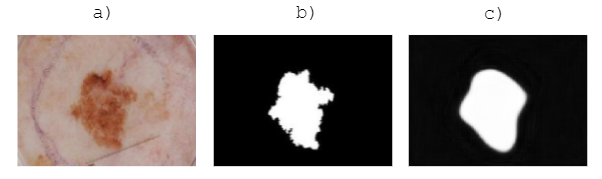
\includegraphics[scale=1.2]{images/border-seg.png}
\caption{Demonstrating the Semantic Pixel-Wise Segmentation (SegNet) results showing the a) original image, b) expert ground-truth and c) SegNet results.} \label{SegNet}
\end{figure}

Results in figure \ref{SegNet} are generated from the architecture using the ISIC 2018 dataset split into 80\% training and 20\% validation images. The accuracy of locating the lesions is 85\%. However, figure \ref{SegNet} represents the border cut-off between skin and skin lesion is accurate to the dataset but inadequate for using the ABCD rules. Finding the border cut-off is vital for measuring ABCD rules \cite{Pereira2020}.

\section{Border extraction}
Box-counting method

\subsection{U-Otsu Threshold}
Otsu threshold is a versatile automatic image thresholding technique meant to separate each pixel between two classes of foreground or background. One of the benefits of this method is that it does not require any training data. The equation \ref{otsu} (within-class variance) describes splitting weights of $w_0(t),w_1(t)$, which are the probabilities divided by the threshold $t$, between 0 to 255. Furthermore, $\sigma_1^2$ and $\sigma_0^2$ are variances of these two classes. The class probability $w$ is computed from the histogram in figure \ref{otsu2}, which is an intensity histogram describing the colour distribution in an image. Measuring the values above and below the generated thresholds splits the image into two classes.

\begin{equation} \label{otsu}
\sigma_w^2(t) = w_0(t)\sigma_1^2(t) + w_1(t)\sigma_2^2(t)
\end{equation}

The histogram is split into two segments with the threshold $t$ of 138 and the corresponding pixel locations to the histogram segment the skin lesion into two classes. Image morphology closing is applied to fill gaps that the threshold missed. On other occasions, the segmentation missed the skin lesion because of a similar colour between the skin and skin lesion. It might be beneficial to combine otsu with SegNet to improve its accuracy while producing a border cut-off. Figure \ref{otsu2} describes the difference between otsu and SegNet.

\begin{figure}
\centering
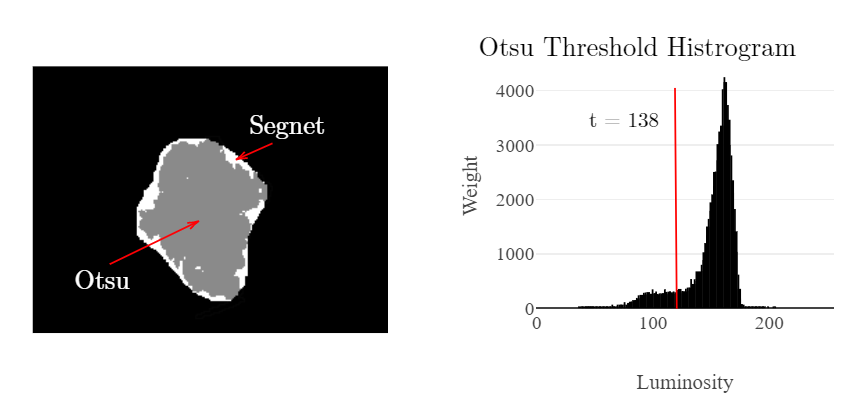
\includegraphics[scale=0.7]{images/otsu3.png}
\caption{Otsu thresholding alongside ground-truth mask, where grey Otsu and white is SegNet. The bar chart shows the histogram with an otsu threshold of 138.} \label{otsu2}
\end{figure}


\subsection{LBPC segmentation}

Local Binary Patterns (LBP) is a texture descriptor commonly used for augmenting the image improving classification accuracy \cite{Pereira2020, Kaya2016}. First, equation \ref{eq1} calculates each pixel, where $p$ (equal to 8) is the number of neighbouring pixels compared to the centre of $c$, and radius of $r$ from the centre. Next, shown in equation \ref{eq2} each value is subtracted counter-clockwise with the centre value and compared to function $S$ where each $gp - gc$, if more than or equal to 0, is equal to 1, and less than 0 is equal to 0. Next, add corresponding values equal to 1 of $gp$ together, changing the centre value, ignoring values of 0. Next, applying a Gaussian kernel of 13-pixel iterations and a standard deviation of 3 removes smaller features that interfere with the segmentation. Finally, applying k-means with a value of 2 subtracts the greyscale and segments the skin lesion from the skin.

\begin{equation} \label{eq1}
LBP(gp_x, gp_y) = \mathlarger{\sum}_{p=0}^{P-1}s\big(gp - gc)2^p
\end{equation}

\begin{equation} \label{eq2}
s\big(x) = 
\begin{cases}
1,\:\:x\geq\:0; \\
0,\:$otherwise$.
\end{cases}
\end{equation}

Figure \ref{fractal1} demonstrates the segmentation of two skin lesions, one with an irregular border and another with a regular border. LBPC is applied to both skin lesions, followed by Gaussian blurring and morphology closing to remove dots. The result is an improved border cut-off compared to the ground-truth in the Ph$^2$ dataset with more corners and ledges. This technique will improve accuracy for measuring border irregularity \cite{Pereira2020}.

\begin{figure}
\centering
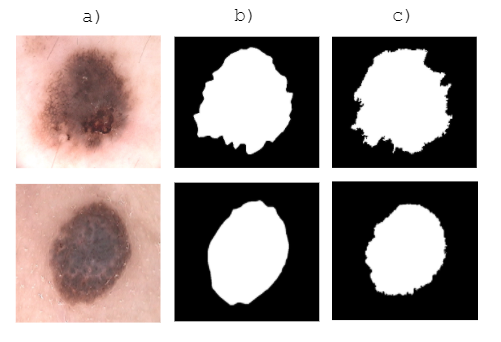
\includegraphics[scale=1.2]{images/borders.PNG}
\caption{Local Binary Pattern Clustering (LBPC) showing the a) original image, b) ground-truth, and c) LBPC. LBPC successfully exaggerates the border cut-off on the skin lesions with regular and irregular borders} 
\end{figure} \label{fractal1}

Validating LBPC is not expected because the goal is to exaggerate the border to improve the classification process of ABCD rules, which it does successfully \cite{Pereira2020, Kaya2016}. For example, the segmentation might not match dataset segmentations but is still essential to classifying ABCD rules. Furthermore, many datasets lack expert border segmentation, an accurate border cut-off between the skin and skin lesions, so comparisons are not always possible.

\subsection{Semantic Pixel-Wise Segmentation}
Semantic pixel-wise segmentation (SegNet) is a machine learning architecture utilising a deep, fully convolutional neural network (DCNN). This network requires training from ground-truth and pre-segmented images for automatic segmentation. SegNet consists of encoding layers, decoding layers, and a pixel-wise classification layer. The encoder layers consist of 3x3 convolutions (including batch normalisation and ReLU), pre-trained filters for classifying features. After some convolutions, the data is down-sampled using a 2x2 pooling layer. Next, decoding layers consist of up-sampling, followed by 3x3 convolutions. Finally, the pixel-wise classification uses a softmax layer to represent each pixel between 0 and 1 based on the previous layers, generating a segmentation mask.

\begin{figure}[hb]
\centering
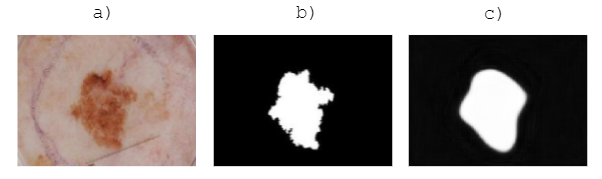
\includegraphics[scale=1.2]{images/border-seg.png}
\caption{Demonstrating the Semantic Pixel-Wise Segmentation (SegNet) results showing the a) original image, b) expert ground-truth and c) SegNet results.} \label{SegNet2}
\end{figure}

Results in figure \ref{SegNet2} are generated from the architecture using the ISIC 2018 dataset split into 80\% training and 20\% validation images. The accuracy of locating the lesions is 85\%. However, figure \ref{SegNet2} represents the border cut-off between skin and skin lesion is accurate to the dataset but inadequate for using the ABCD rules. Finding the border cut-off is vital for measuring ABCD rules \cite{Pereira2020}.

\section{Experimental results}
Both statistical models of LBPC and Otsu threshold generated accurate border cut-off as compared to the machine learning approach SegNet. Measuring border cut-off exaggerates irregular borders successfully, making it helpful in detecting border irregularities and possibly with other ABCD rules. It might be beneficial to combine SegNet and LBPC by using SegNet to find the skin lesions' location, followed by adjusting the border cut-off using LBPC.


